%@def.tex
\documentclass[landscape]{slides}
\usepackage[warn]{mathtext}
\usepackage[T2A]{fontenc}
\usepackage[utf8]{inputenc}
\usepackage[english, russian]{babel}
\usepackage{indentfirst}
\usepackage{amsmath, amsfonts, amssymb}
\usepackage{geometry}
\usepackage{hyperref}
\usepackage{wrapfig}
\geometry{top=2cm}
\geometry{left=3cm}
\geometry{right=2cm}
\geometry{bottom=2cm}
\usepackage{color}
\usepackage{multirow}
\usepackage{lscape}
\usepackage{wrapfig}
\usepackage{graphicx}
\usepackage{epstopdf}
\usepackage{tikz}
\usepackage{tikz-3dplot}
\usetikzlibrary{arrows}
\usetikzlibrary{calc}

\renewcommand{\vec}{\overline}
\renewcommand{\phi}{\varphi}

\graphicspath{{pics/}}

\makeatletter
\newcommand{\nextverbatimspread}[1]{%
    \def\verbatim@font{%
        \linespread{#1}\normalfont\ttfamily% Updated definition
            \gdef\verbatim@font{\normalfont\ttfamily}}% Revert to old definition
}
\makeatother

\newenvironment{mintemize}{%
    \vspace{-1.5em}
    \begin{itemize}
        \setlength\itemsep{-0.2em}
}
{
    \end{itemize}
    \vspace{-1em}
}

\newenvironment{cslide}{%
    \begin{slide}
    \begin{center}
}
{
    \end{center}
    \end{slide}
}

\makeatletter
\def\sltop{\let\@topfil\relax}
\makeatother

\newenvironment{tslide}[1]{%
    \begin{slide}
    \sltop
    {\large\textbf{#1}}
}
{ \end{slide} }


\begin{document}

\begin{cslide}
    
\includegraphics[width=3cm]{mai.eps}

    \large\textbf{ Разработка алгоритмов управления
    массивом беспилотных летательных аппаратов
    с целью построения информационного поля
    участка местности}

    \vfill

    \begin{flushright}
    \small Выполнил студент гр. 07-608 Бутко О.А.

    \small Руководитель Жидков В.Н.
    \end{flushright}

    \vfill

    \small Москва, 2015
\end{cslide}

\begin{tslide}{Постановка задачи}

Создание алгоритма исследования местности,
формирования цифровой карты, а также поддержание
ее в актуальном состоянии, посредством МБПЛА,
включает следующие этапы:
\begin{itemize}
\item Формализация модели цифровой карты
\item Анализ минимальных требований аппаратного состава МБПЛА для решения задачи построения карты
\item Формализация модели МБПЛА
\item Разработка алгоритма распределенных вычислений для обработки больших объемов информации
\item Разработка алгоритма обхода местности
\item Разработка схемы и программного комплекса имитационного моделирования для различных вариантов алгоритма обхода:
    \begin{itemize}
    \item распределение подгрупп юнитов по регионам карты
    \item выбор случайной точки в пространстве карты
    \end{itemize}
\item Проведение имитационного моделирования, обобщение и анализ полученных результатов.
\end{itemize}

\end{tslide}

\begin{tslide}{Формализация модели цифровой карты}
\end{tslide}

\begin{tslide}{Анализ минимальных требований аппаратного состава
МБПЛА для решения задачи построения карты}

    \begin{wrapfigure}{r}{0.3\textwidth}
        \vspace{-1cm}
        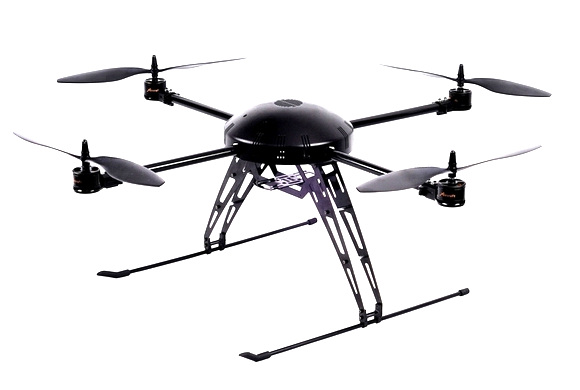
\includegraphics[width=\linewidth]{X650.jpg}
        \vspace{-2.8cm}
    \end{wrapfigure}

    За основу была взята концепция БПЛА с вертикальным взлётом.
    Будем считать, что:
    \begin{itemize}
    \item каждый юнит знает свой фазовый вектор
    \item каждый юнит знает фазовые вектора остальных юнитов системы
    \item на борту юнита установлена аппаратура, позволяющая получать карту глубин
    \item у каждого юнита есть возможность читать и писать в карту местности
    \end{itemize}

\end{tslide}

\begin{tslide}{Что такое массив БПЛА}

    Массив БПЛА -- группа однотипны, сверхлёгких, дешёвых БПЛА,
    значительно превышающая по количеству классические группы

    Юнит -- элемент массива БПЛА

    Количество юнитов в системе может исчисляться тысячами
\end{tslide}

\begin{tslide}{Для чего нужен МБПЛА}

    Построение трёхмерной динамической \newline
        карты неизвестной местности

    \vfill
    \begin{center}
    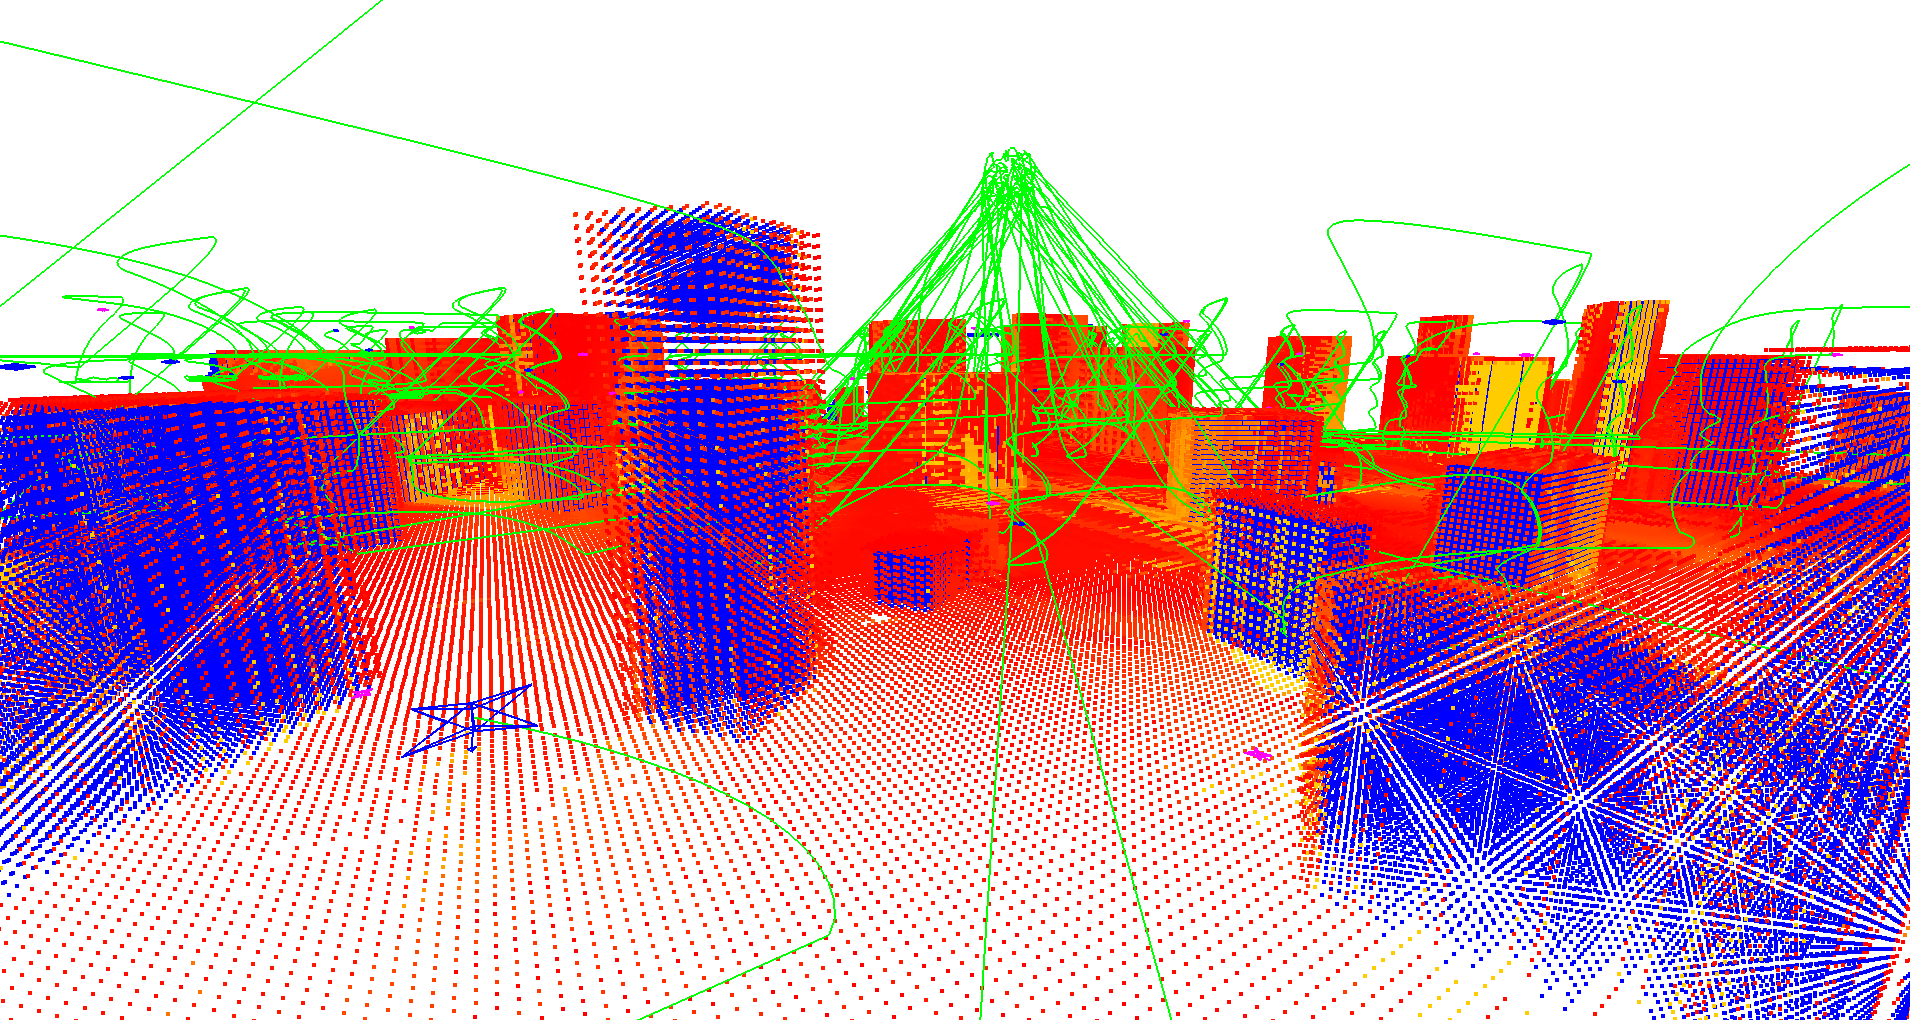
\includegraphics[width=.9\linewidth]{s50s_map2.png}
    \end{center}
    \vfill
\end{tslide}

\begin{tslide}{Для чего нужен МБПЛА}

    Исследование и построение карты помещений
    \vfill

    \begin{center}
    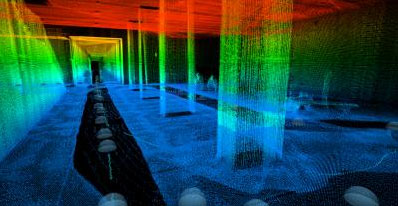
\includegraphics[width=.9\linewidth]{mapInside.jpg}
    \end{center}
    \vfill

\end{tslide}

\begin{tslide}{Модель карты местности}

    Предполагается что участок местности ограничен по ширине,
    глубине и высоте.
    Он разбивается на прямоугольные сектора, каждый из которых хранит
    информацию об единице объёма
    \vfill

    \begin{center}
    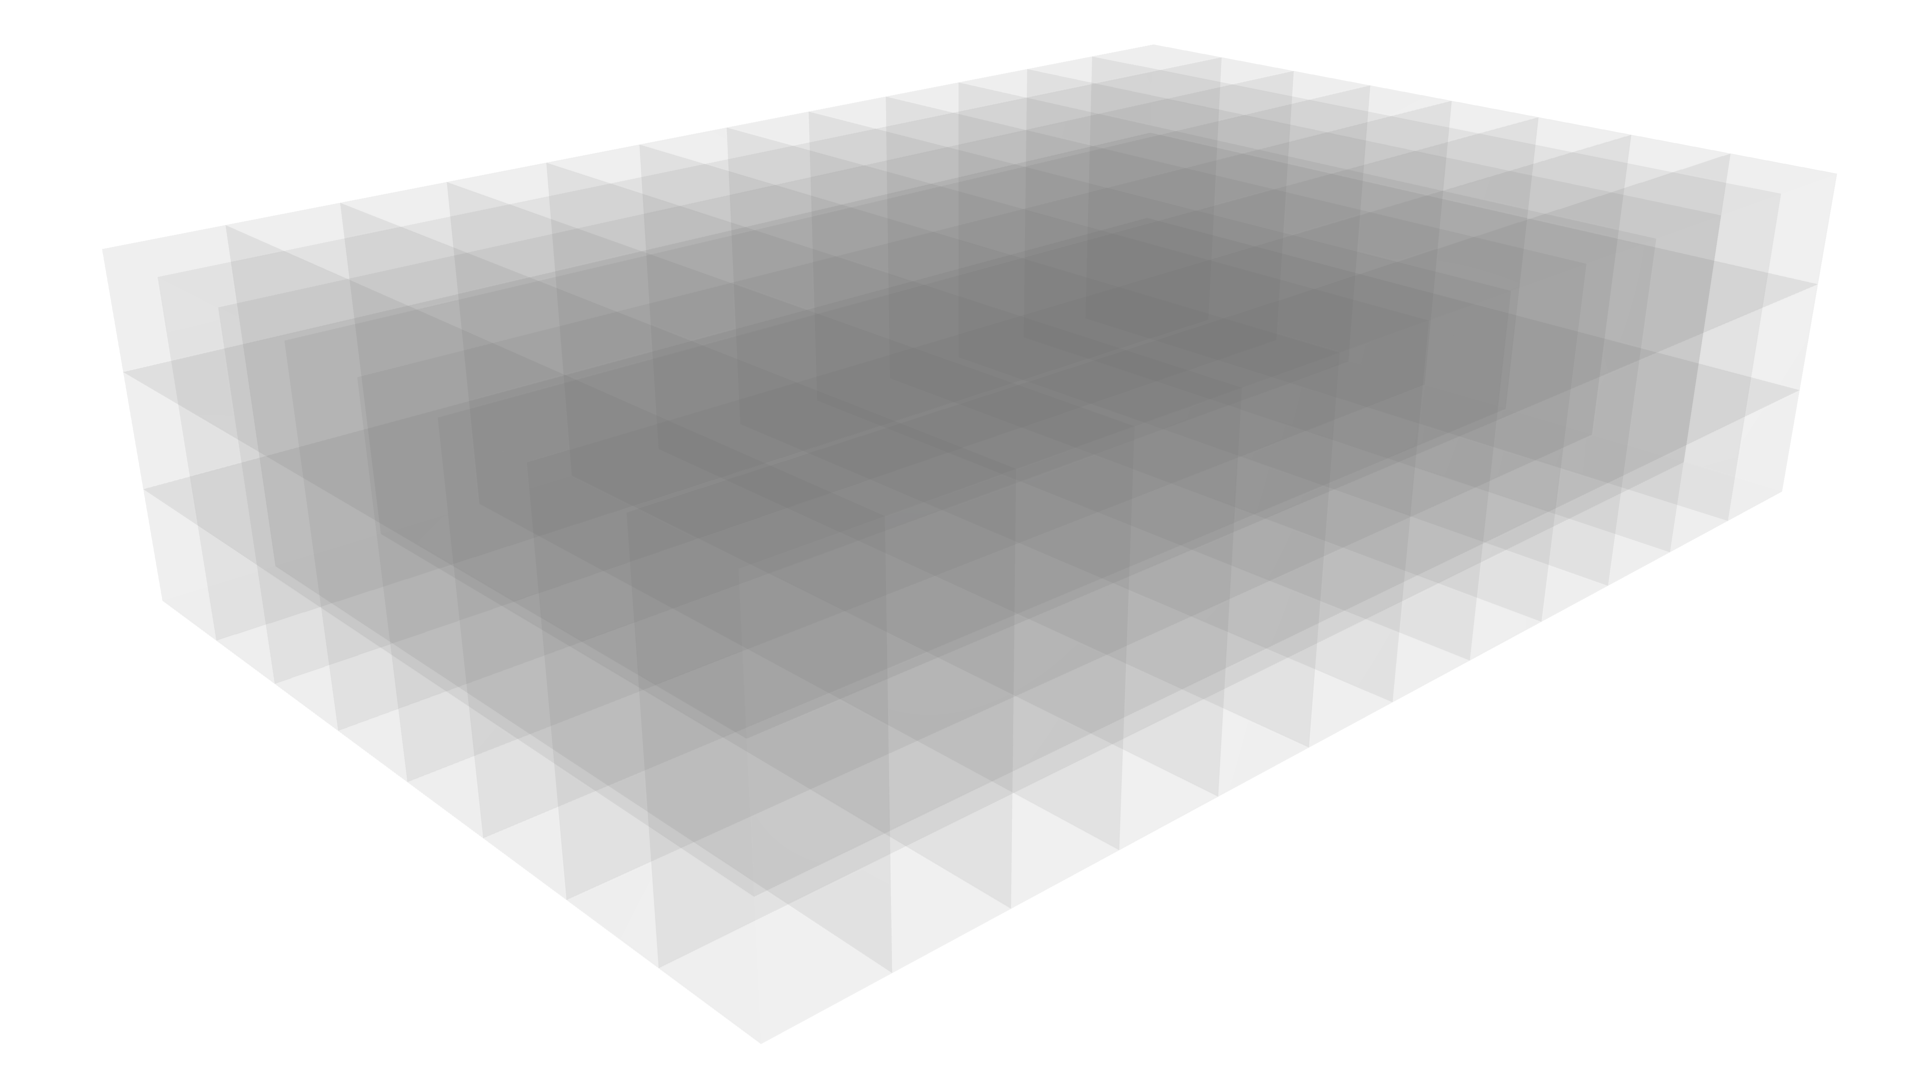
\includegraphics[width=.8\linewidth]{map.png}
    \end{center}
    \vfill

\end{tslide}

\begin{tslide}{Реализация карты местности}

    Реализация карты представляет собой 1-мерный массив,
    к которому можно обратиться с помощью трёх индексов-координат.
    Так же для карты имеется матрица трансформации координат
    из локальных (индексов) в глобальные (метры).
    \vfill

    \begin{center}
    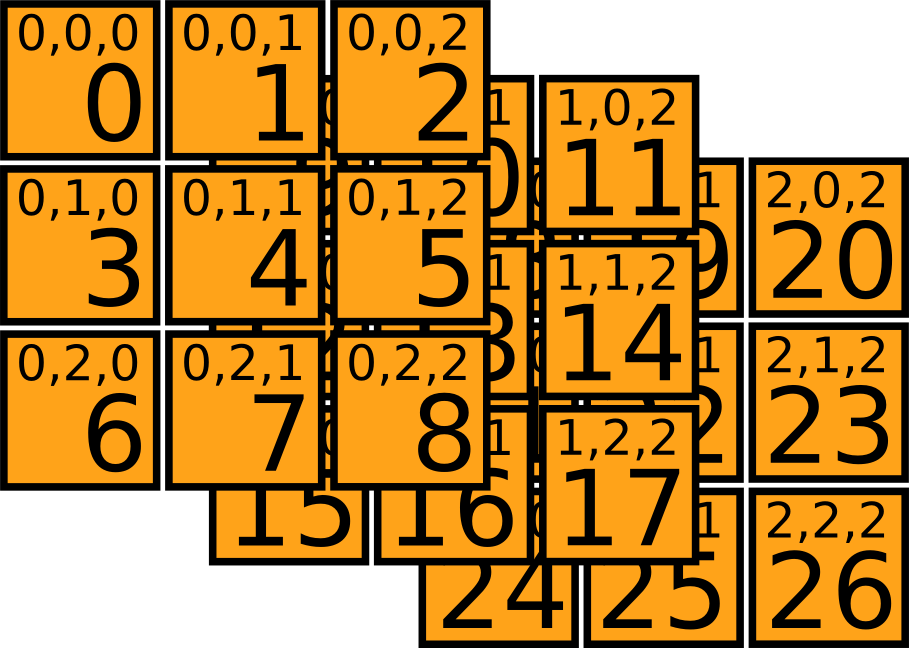
\includegraphics[width=.6\linewidth]{mapRealisation.png}
    \end{center}
    \vfill

\end{tslide}

\begin{tslide}{Реализация карты местности}

    Каждый сектор хранит:

    \begin{mintemize}
    \item {\Large\verb|N|} -- сколько раз был исследован сектор
    \item {\Large\verb|T|} -- когда было произведенно последнее исследование
    \item {\Large\verb|val|} -- результат исследования (занят ли сектор)
    \item {\Large\verb|align|} -- поле для выравнивания до 16 байт
    \end{mintemize}

    \vfill

    \begin{center}
    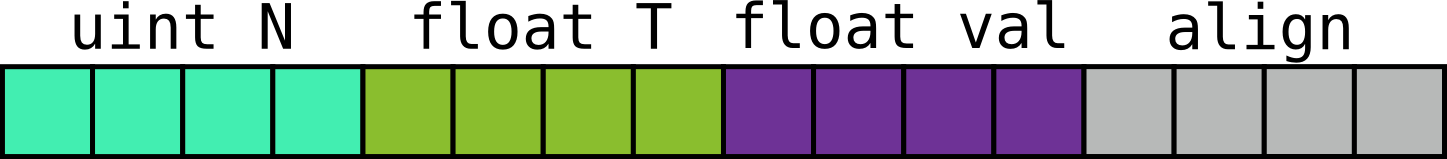
\includegraphics[width=\linewidth]{mapData.png}
    \end{center}

    \vfill

\end{tslide}

\begin{tslide}{Модель единицы массива}
    
    \begin{wrapfigure}{r}{0.3\textwidth}
        \vspace{-1cm}
        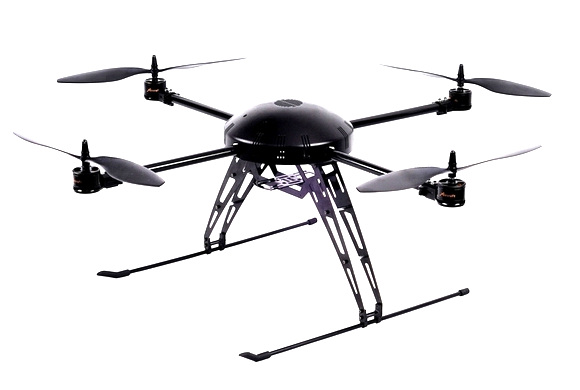
\includegraphics[width=\linewidth]{X650.jpg}
        \vspace{-2.8cm}
    \end{wrapfigure}

    За основу была взята концепция БПЛА с вертикальным взлётом

    Дифференциальное уравнение движения:
    $$
    \left\{
        \begin{array}{l l}
        \dot{\vec{p}}  & = \vec V \\
        \dot{\vec{V}}  & = \vec a + \vec g
        \end{array}
    \right.
    $$

    где: 

    $\vec p, \vec V$ -- координаты и скорость юнита
    
    $\vec g$ -- ускорение свободного падения

    $\vec a = \frac{1}{m} \sum_{i=1}^N F_i$ -- ускорение от действующих на юнит сил

\end{tslide}

\begin{tslide}{Модель единицы массива}
    
    Действующих на юнит силы

    \tikzstyle{every picture}+=[
        axis/.style={black},
        vector/.style={->,line width=1mm,black},
        help/.style={gray,thin,dashed},
        rot/.style={tdplot_rotated_coords}
    ]

    \def\dot{circle[radius=1mm]}
    \def\P{1.9}
    \def\Pm{1.6}
    \def\Pmm{0.5}
    \def\Vrot{10}
    \def\fnlen{4}
    \def\ftlen{3}
    \def\dst{8}

    \begin{center}
    \tdplotsetmaincoords{0}{0}
    \begin{tikzpicture}[scale=1.6,tdplot_main_coords]
        \tdplotsetrotatedcoords{85}{60}{-50}

        \draw[rot,vector,blue] (0,0) -- (\dst,0);
        \node[rot,below right] at (6,0) {$\vec F_\text{упр}$};

        \draw[rot,vector] (0,0) -- (\Vrot:5) node[above] {$\vec V$};
        \draw[rot,vector,red] (0,0) -- (180+\Vrot:3);
        \node[rot,below] at (180+\Vrot:3) {$\vec X_0$};
        \draw[rot,vector,green] (0,0) -- (-\fnlen,\ftlen,0);
        \node[rot,above left] at (-\fnlen,\ftlen) {$\vec F_{\text{кор}}$};

        \draw[rot,help] (-\fnlen,\ftlen) -- (\dst-\fnlen,\ftlen);
        \draw[rot,help] (\dst,0) -- (\dst-\fnlen,\ftlen);
        \draw[rot,help] (0,0) -- (\dst-\fnlen,\ftlen);
        \draw[rot,vector] (0,0) -- ($(\dst-\fnlen,\ftlen)+(180+\Vrot:3)$) node (S) {};
        \draw[rot,help] (180+\Vrot:3) -- (S);
        \draw[rot,help] (\dst-\fnlen,\ftlen) -- (S);

        \node[rot,left] at (S) {$\vec F$};
        \fill[rot,black] (0,0) \dot node[below] {$O$};

    \end{tikzpicture}
    \end{center}
    \begin{itemize}

    \item $\vec X_0 = C_{x0}\frac{-\vec V \rho |V|}{2} S$ -- сила сопротивления воздуха
    \item $\vec F_\text{упр}$ -- управляющее воздействие
    \item $\vec F_\text{кор}$ -- коррекция по ближайшим опасным точкам
    \end{itemize}

\end{tslide}

\begin{tslide}{Модель единицы массива}

    У каждого юнита на борту имеется сенсор измеряющий \newline
    <<карту глубин>> с определённым разрешением и дальностью
    \vfill
    
    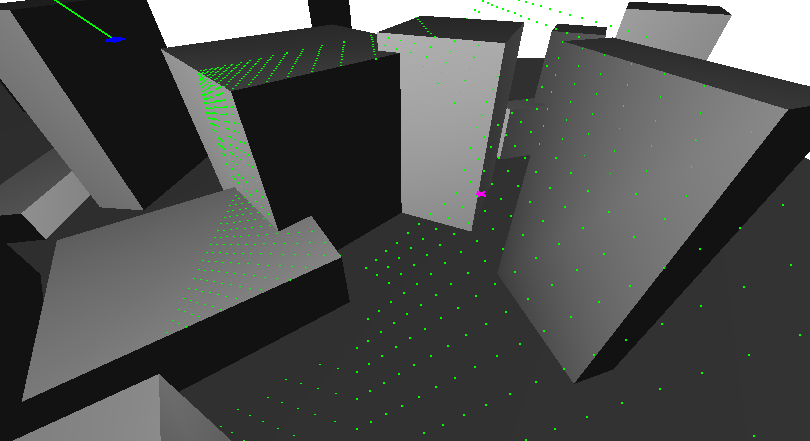
\includegraphics[width=\linewidth]{simDepthMap2.png}
    \vfill

\end{tslide}

\begin{tslide}{Заполнение карты}

    Получаем карту глубин

    \vfill
    \begin{center}
    
\includegraphics[width=.7\linewidth]{depthView.png}
    \end{center}
    \vfill

\end{tslide}

\begin{tslide}{Заполнение карты}

    С помощью обратной матрицы перспективной трансформации
    переводим каждую точку на карте глубин в точку в пространстве

$$
\vec U = \left( \begin{array}{c c c c}
        \frac{1}{ R \cdot \tan( \frac{1}{2} A ) } & 0 & 0 & 0 \\
        0 & \frac{1}{ \tan( \frac{1}{2} A ) } & 0 & 0 \\
        0 & 0 & \frac{ z_{n} + z_{f} }{ z_{n}-z_{f} } & \frac{ 2 \cdot z_{n} \cdot z_{f} }{ z_{n} - z_{f} } \\
        0 & 0 & -1 & 0 \end{array} \right)^{-1}
    \left( \begin{array}{c} x \\ y \\ depth \\ 1 \end{array} \right)
$$

$$\vec P = \frac{( X_U, Y_U, Z_U )^T}{ W_U } $$

\end{tslide}

\begin{tslide}{Заполнение карты}

    Кадждую полученную точку и координаты камеры юнита
    приводим к системе координат карты и строим отрезок

    \vfill

    \begin{center}
    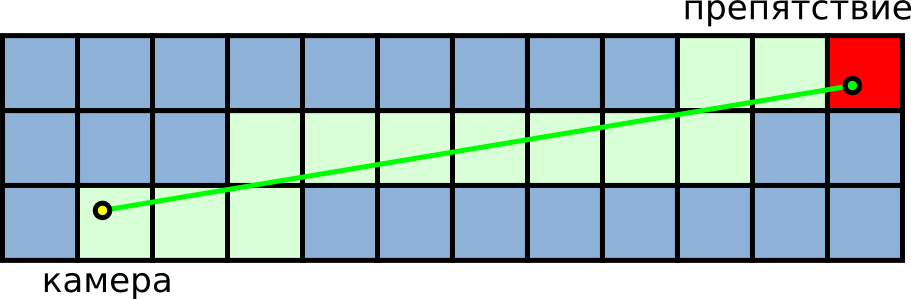
\includegraphics[width=\linewidth]{mapRaster.png}
    \end{center}

    \vfill

\end{tslide}

\begin{tslide}{Коррекция по ближайшим опасным точкам}

    \tikzstyle{every picture}+=[
        axis/.style={black},
        vector/.style={->,line width=1mm,black},
        help/.style={gray,thin,dashed},
        rot/.style={tdplot_rotated_coords}
    ]

    \def\dot{circle[radius=0.5mm]}
    \def\P{1.9}
    \def\Pm{1.6}
    \def\Pmm{0.5}
    \def\Vrot{20}
    \def\fnlen{5}
    \def\ftlen{2}
    \def\dst{8}

    \begin{center}
    \tdplotsetmaincoords{0}{0}
    \begin{tikzpicture}[scale=1.6,tdplot_main_coords]
        \tdplotsetrotatedcoords{85}{60}{-50}
        \fill[rot,red] (\dst,  0,  0) \dot;
        \fill[rot,red] (\dst, .5,  0) \dot;
        \fill[rot,red] (\dst,-.5,  0) \dot;
        \fill[rot,red] (\dst, .5, .5) \dot;
        \fill[rot,red] (\dst,-.5, .5) \dot;
        \fill[rot,red] (\dst,  0, .5) \dot;
        \fill[rot,red] (\dst,  0,-.5) \dot;
        \fill[rot,red] (\dst, .5,-.5) \dot;
        \fill[rot,red] (\dst,-.5,-.5) \dot;

        \fill[rot,black] (0,0,0) \dot node[below] {$O$};

        \draw[rot,vector] (0,0,0) -- (\dst,0,0);
        \node[rot,above] at (6,0,0) {$\vec D$};
        \draw[rot,vector] (0,0,0) -- (1,0,0);
        \node[rot,below] at (1,0,0) {$\vec e_D$};

        \draw[rot,vector] (0,0,0) -- (\Vrot:5) node[above] {$\vec V$};
        \draw[rot,vector] (0,0,0) -- (\Vrot:1) node[above] {$\vec e_V$};
        \draw[rot,vector,help] (0,0,0) -- (0,0,3);
        \node[rot,left] at (0,0,3) {$\vec U$};
        \draw[rot,vector,red] (0,0,0) -- (-\fnlen,0,0);
        \draw[rot,vector,red] (0,0,0) -- (-1,0,0);
        \node[rot,below left] at (-\fnlen,0,0) {$\vec F_N$};
        \node[rot,below] at (-1,0,0) {$\vec N$};
        \draw[rot,vector,green] (0,0,0) -- (0,\ftlen,0);
        \draw[rot,vector,green] (0,0,0) -- (0,1,0);
        \node[rot,above left] at (0,\ftlen,0) {$\vec F_T$};
        \node[rot,above] at (0,1,0) {$\vec T$};
        \draw[rot,vector,blue] (0,0,0) -- (-\fnlen,\ftlen,0);
        \node[rot,above left] at (-\fnlen,\ftlen,0) {$\vec F_\text{кор}$};

        \draw[rot,help] (0,\ftlen,0) -- ++(-\fnlen,0,0) -- ++(0,-\ftlen,0);

        \draw[rot,help] (0,0,\P) -- ++(0:\P) -- ++(0,0,-\P);
        \draw[rot,help] (0,0,\P) -- ++(\Vrot:\P) -- ++(0,0,-\P);
        \draw[rot,help] (0,\Pm,0) -- ++(\Pm,0,0) -- ++(0,-\Pm,0);
        \draw[rot,help] (-\Pmm,0,0) -- ++(0,\Pmm,0) -- ++(\Pmm,0,0);
    \end{tikzpicture}
    \end{center}

    К ближайшим опасным точкам относятся заполненные сектора карты и
    юниты системы.

    Направление тангенсальной компоненты определяется по направлению 
    текущей скорости.

\end{tslide}

\begin{tslide}{Управляющее воздействие}

    Управляющее воздействие определяется положением целевой
    точки

    \def\sum{ circle[radius=2mm] }

    \tikzset{%
    block/.style    = {draw, thick, rectangle,
                        minimum height = 2em,
                        minimum width = 2em},
    input/.style    = {coordinate,circle,draw,scale=0.3,node distance=6cm}, % Input
    output/.style   = {coordinate}, % Output
    cross/.style={path picture={
                    \draw[black]
                (path picture bounding box.south east) -- (path picture bounding box.north west) (path picture bounding box.south west) -- (path picture bounding box.north east);
                }},
    sum/.style      = {draw,circle,cross} % Adder
    }

    \begin{center}
    \begin{tikzpicture}[auto, thick, node distance=3cm, >=triangle 45,scale=1]
        \draw
        node[input] (input1) {} 
        node[sum, right of=input1] (suma1) {}
        node[input, below of=suma1] (input2) {} 
        node[block, right of=suma1] (PID) {$PID$};

        \draw[->] (input1) -- node[above left] {$\vec X_\text{т}$} (suma1);
        \draw[->] (input2) -- node[below left] {$\vec X_\text{ц}$} (suma1);
        \draw[->] (input2) -- node[above right] {$-$} (suma1);
        \draw[->] (suma1) -- node {} (PID);
        \draw[->] (PID) -- node[above right] {$\vec F_\text{упр}$} +(3cm,0);

    \end{tikzpicture}
    \end{center}

    Было выбрано 3 вариации выбора целевых точек:
    \begin{itemize}
        \item Распределение по регионам карты подгрупп юнитов
        \item Поиск ближайших неизведанных регионов
        \item Выбор случайной точки в пределах карты
    \end{itemize}

\end{tslide}

\begin{tslide}{Распределение по регионам карты подгрупп юнитов}


    \vfill

    \begin{center}
    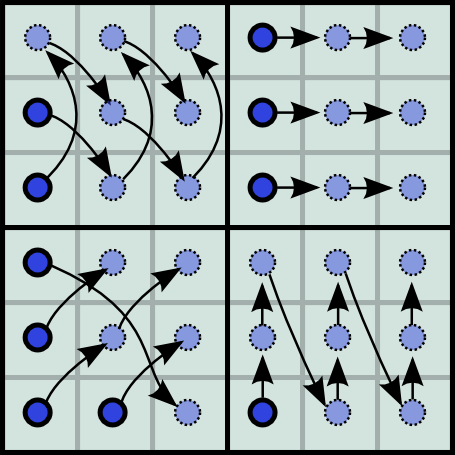
\includegraphics[width=.6\linewidth]{unitSerialMove.png}
    \end{center}

    \vfill

\end{tslide}

\begin{tslide}{Поиск ближайших неизведанных регионов}

    \vfill

    \begin{center}
    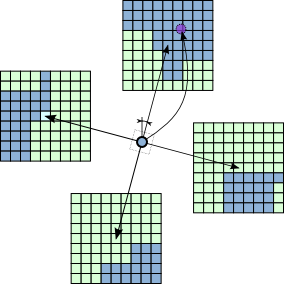
\includegraphics[width=.6\linewidth]{unitFineMove.png}
    \end{center}

    \vfill

\end{tslide}

\begin{tslide}{Момент смены целевой точки}

    \tikzstyle{startnode} = [circle,minimum size=.5cm,fill=black]
    \tikzstyle{stepnode} = [draw,rectangle, minimum height=0.7cm,
                text centered, rounded corners]
    \tikzstyle{endnode} = [circle,minimum size=.5cm,fill=white,draw=black]
    \tikzstyle{statnode} = [diamond,aspect=3,draw,text badly centered,inner sep=0pt]

    \begin{wrapfigure}{r}{0.3\linewidth}
    \begin{tikzpicture}[>=triangle 45,shorten >= 0pt,auto,node distance=2cm]

        \node[startnode] (0) {};
        \node[stepnode] (1) [below of=0] {\verb|n++|};
        \node[statnode] (2) [below of=1] {\verb|n >= K|};
        \node[endnode] (r1) [right=2cm of 2] {};
        \node[statnode] (3) [below of=2] {\verb|D < limit|};
        \node[endnode] (r2) [below of=r1] {};
        \node[stepnode] (4) [below of=3] {\verb|n=0|};
        \node[stepnode] (5) [below of=4] {\verb|choiseTarget()|};
        \node[endnode] (6) [below of=5] {};

        \path[->]
        (0) edge (1) 
        (1) edge (2) 
        (2) edge (3)
        (3) edge (4)
        (2) edge node[above] {$\text{нет}$} (r1)
        (3) edge node[above] {$\text{нет}$} (r2)
        (4) edge (5)
        (5) edge (6);

    \end{tikzpicture}

    \end{wrapfigure}

    \verb|n| -- счётчик шагов

    \verb|K| -- минимальное количество шагов, необходимое для смены целевой
                точки

    \verb|D| -- дисперсия длин вектор последних координат

    \verb|limit| -- порог для значения дисперсии

\end{tslide}

\begin{tslide}{Программно-математическое обеспечение}

    В ПМО можно выделить 3 основные части:
    \begin{itemize}
        \item Базовая -- работа с векторами, матрицами, системы
    взаимодействия классов, управление памятью и тд

        \item Графическая -- оконная система, классовые обёртки
            для работы с \verb|OpenGL|

        \item Симуляция МБПЛА
    \end{itemize}

    Гетерогенные вычисления с использованием \verb|OpenCL| нельзя
    полностью отнести к симуляции МБПЛА, так как они тесно связанны
    с графической частью.

\end{tslide}

\begin{tslide}{Программно-математическое обеспечение}

    \centering
    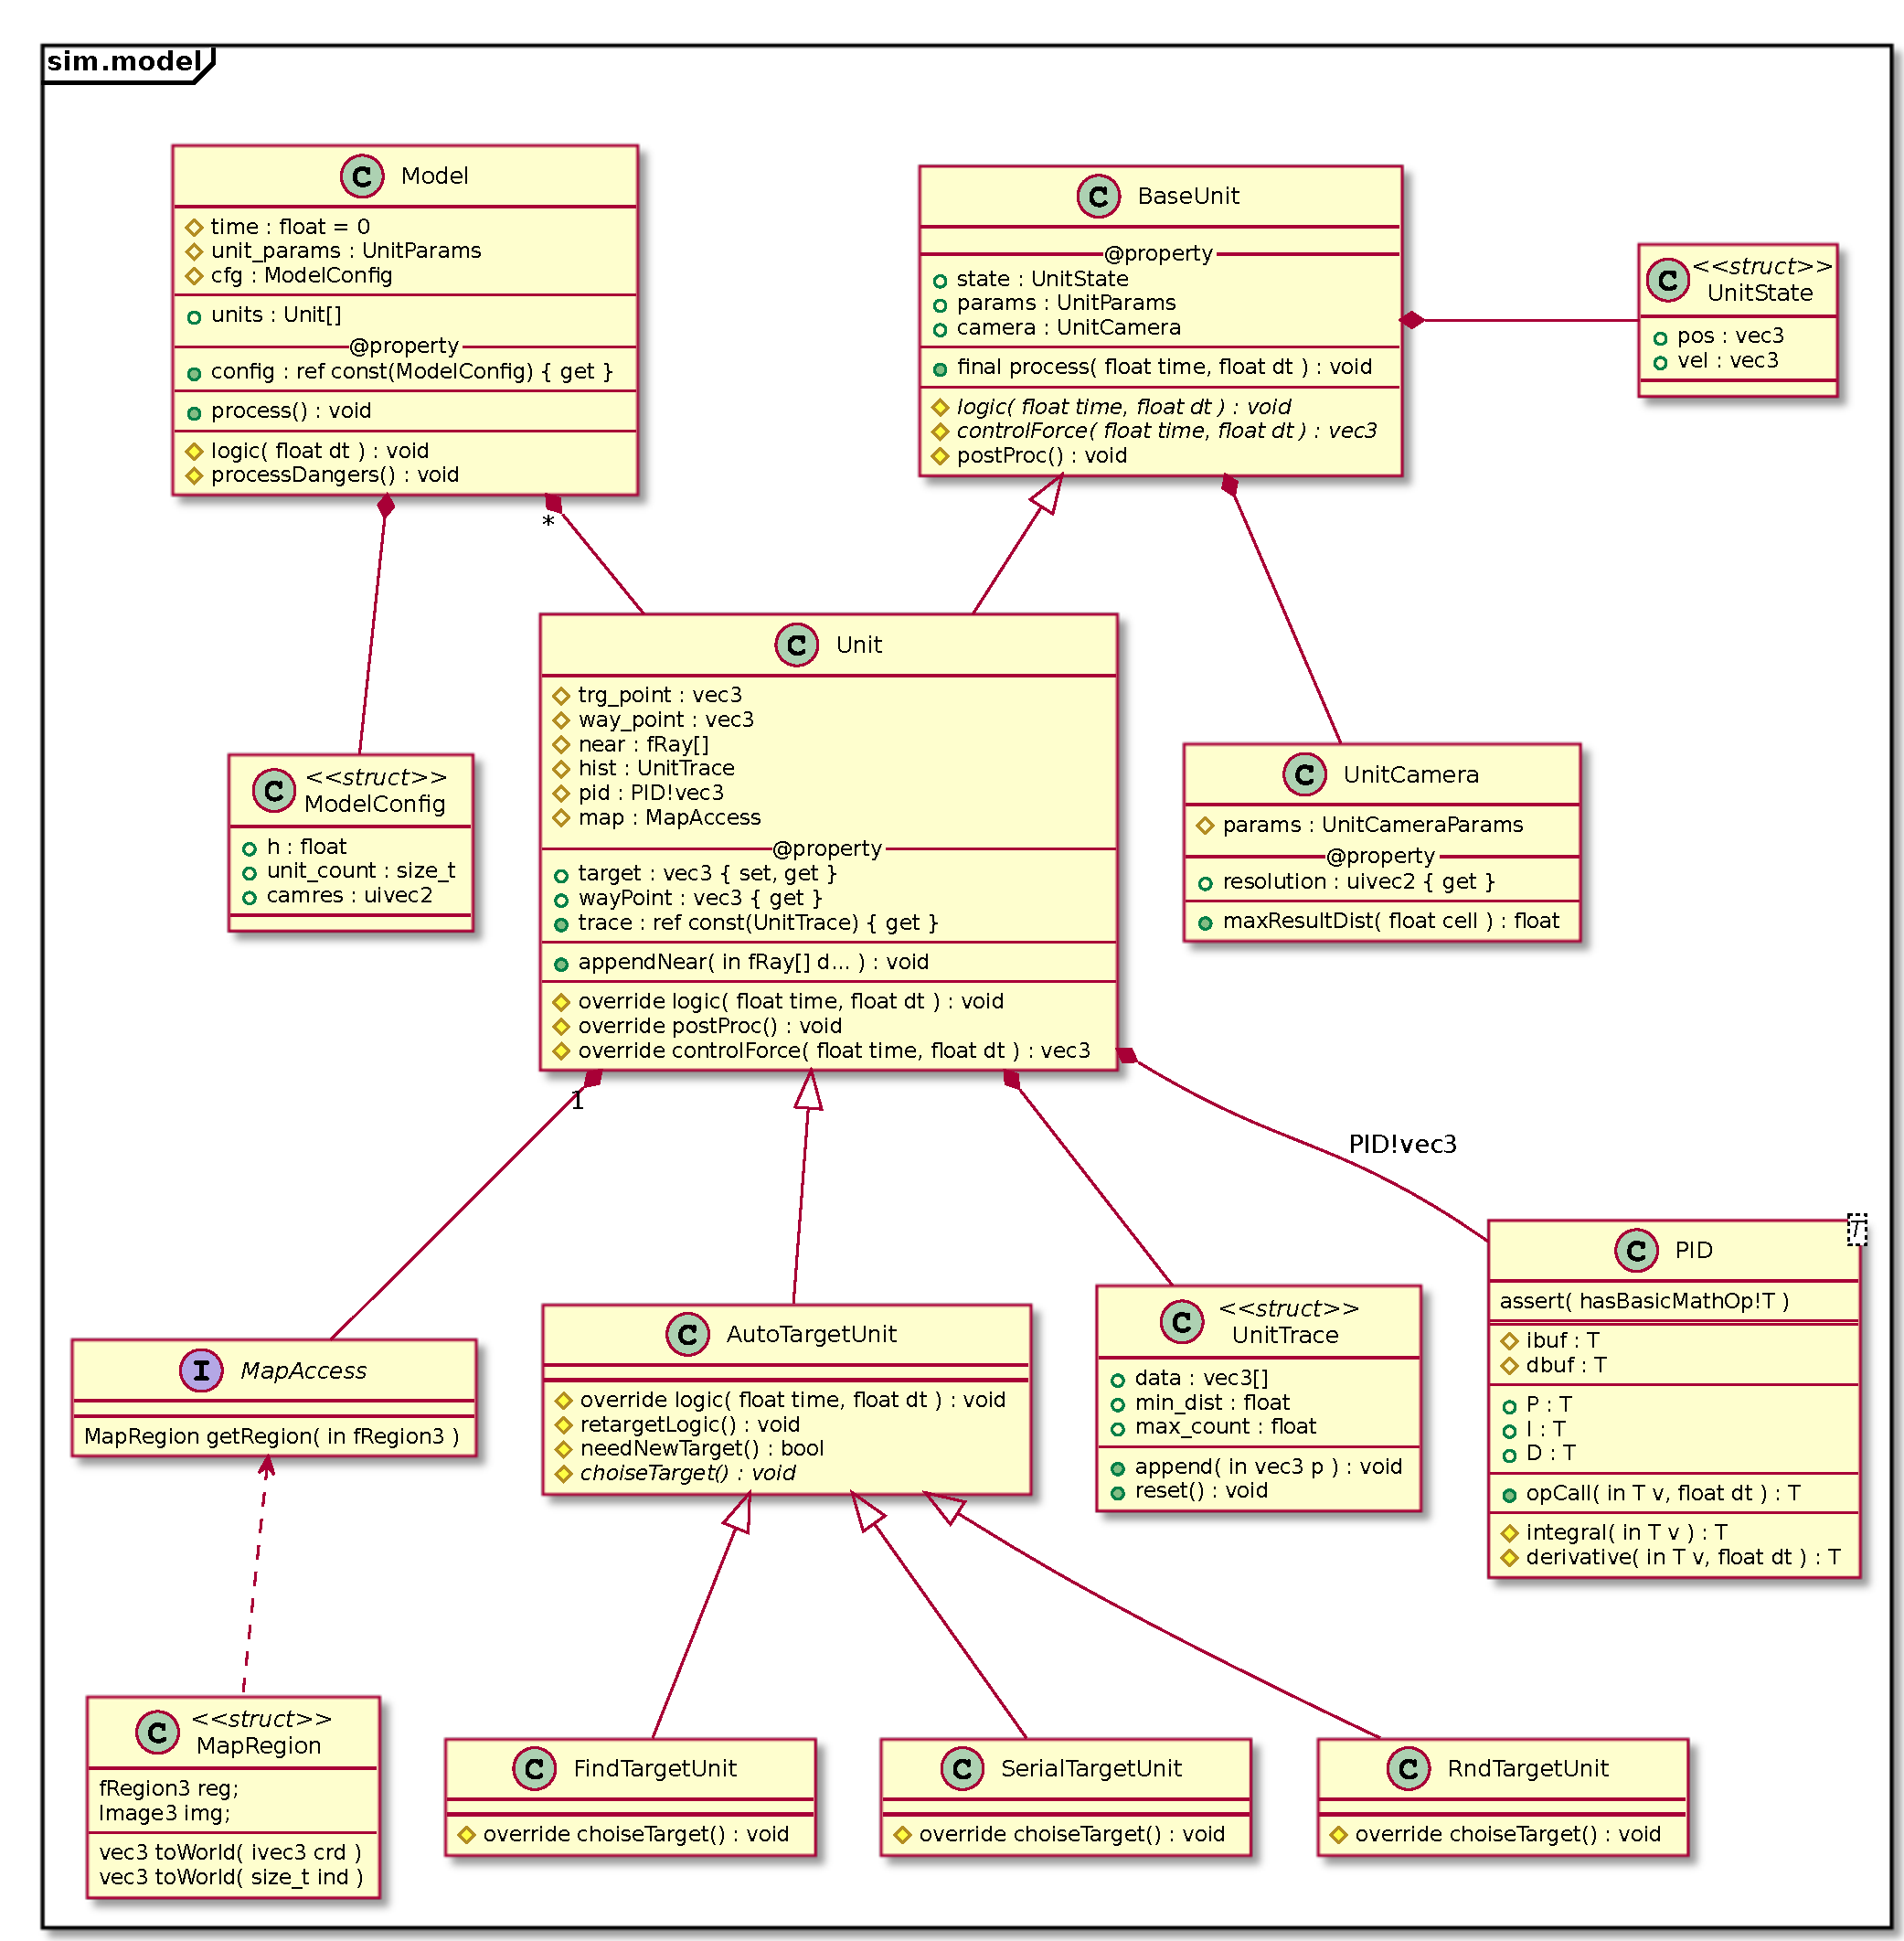
\includegraphics[width=.6\linewidth]{model_uml.eps}

\end{tslide}

\begin{tslide}{Результаты экспериментов}

    \vfill

    \begin{center}
    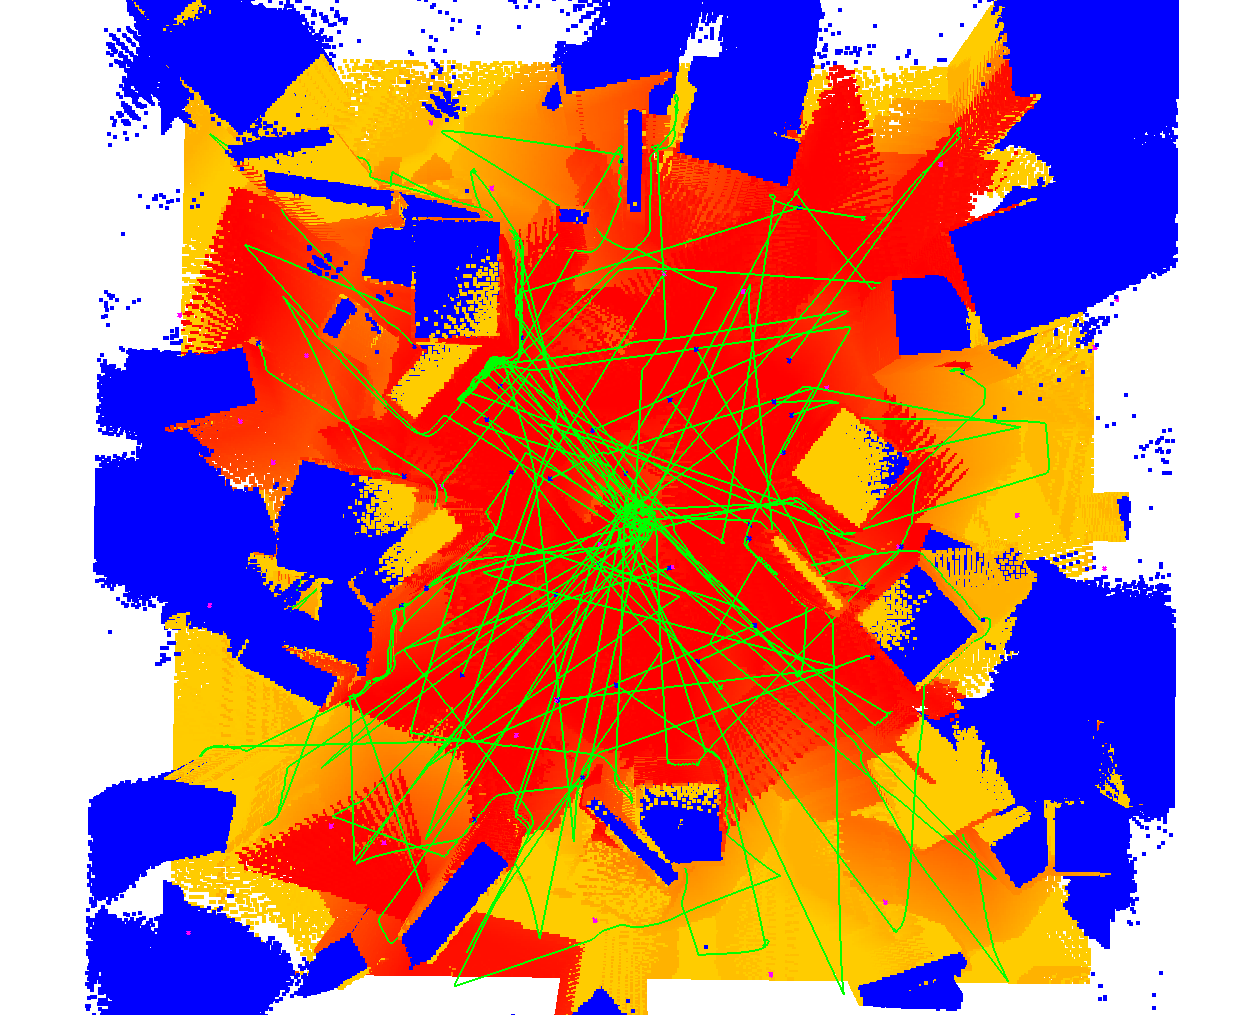
\includegraphics[width=.3\linewidth]{s50rm_map.png}
    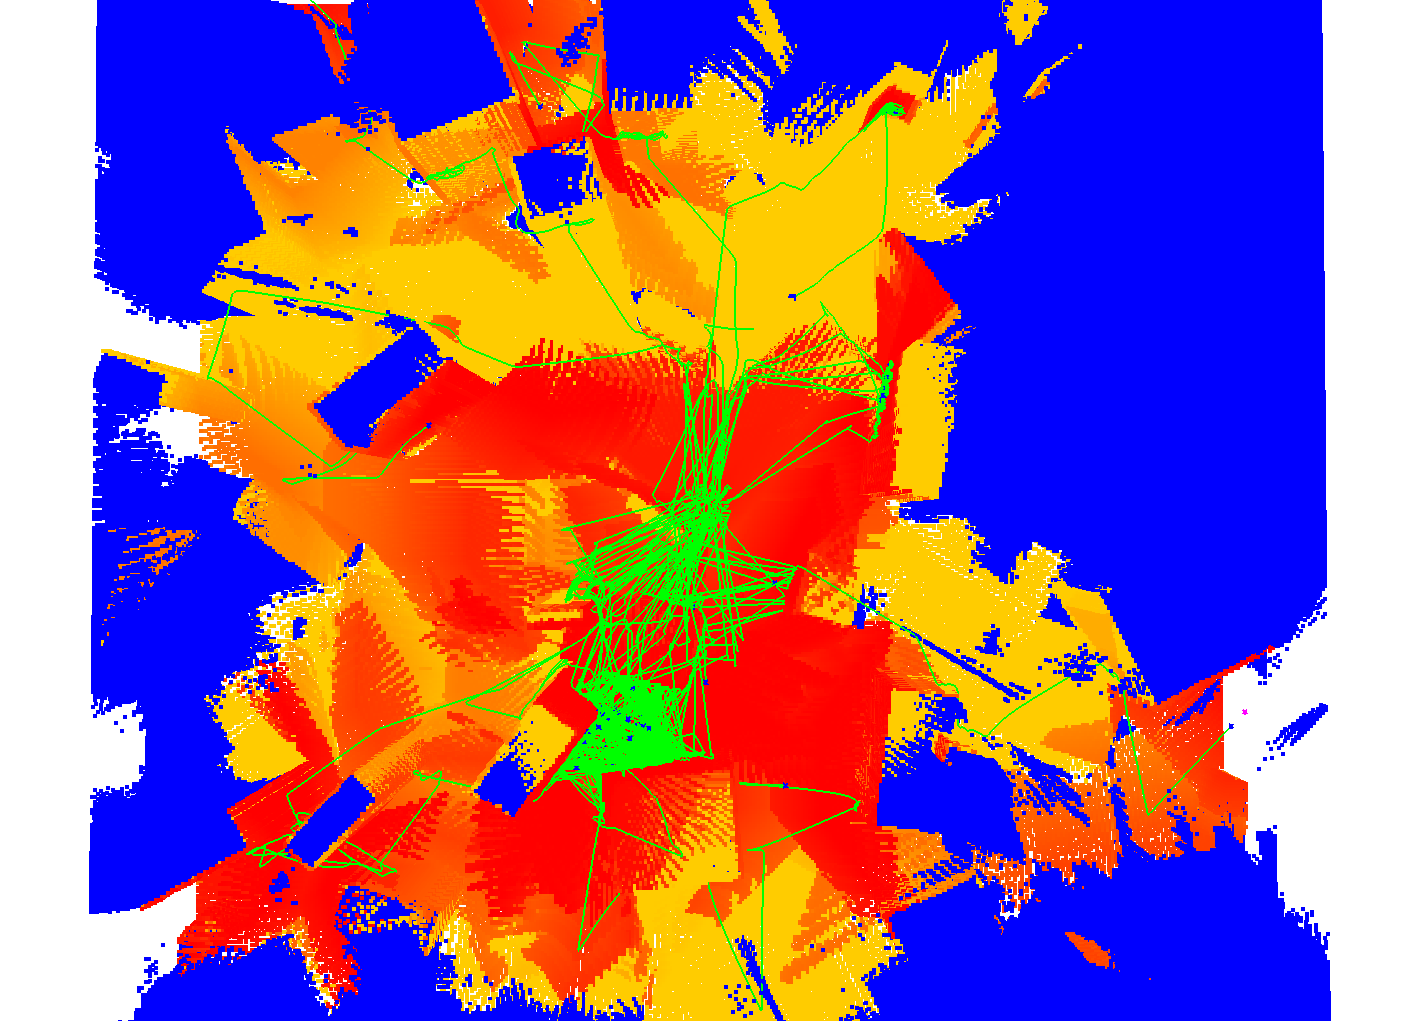
\includegraphics[width=.3\linewidth]{s50f4r_map.png}
    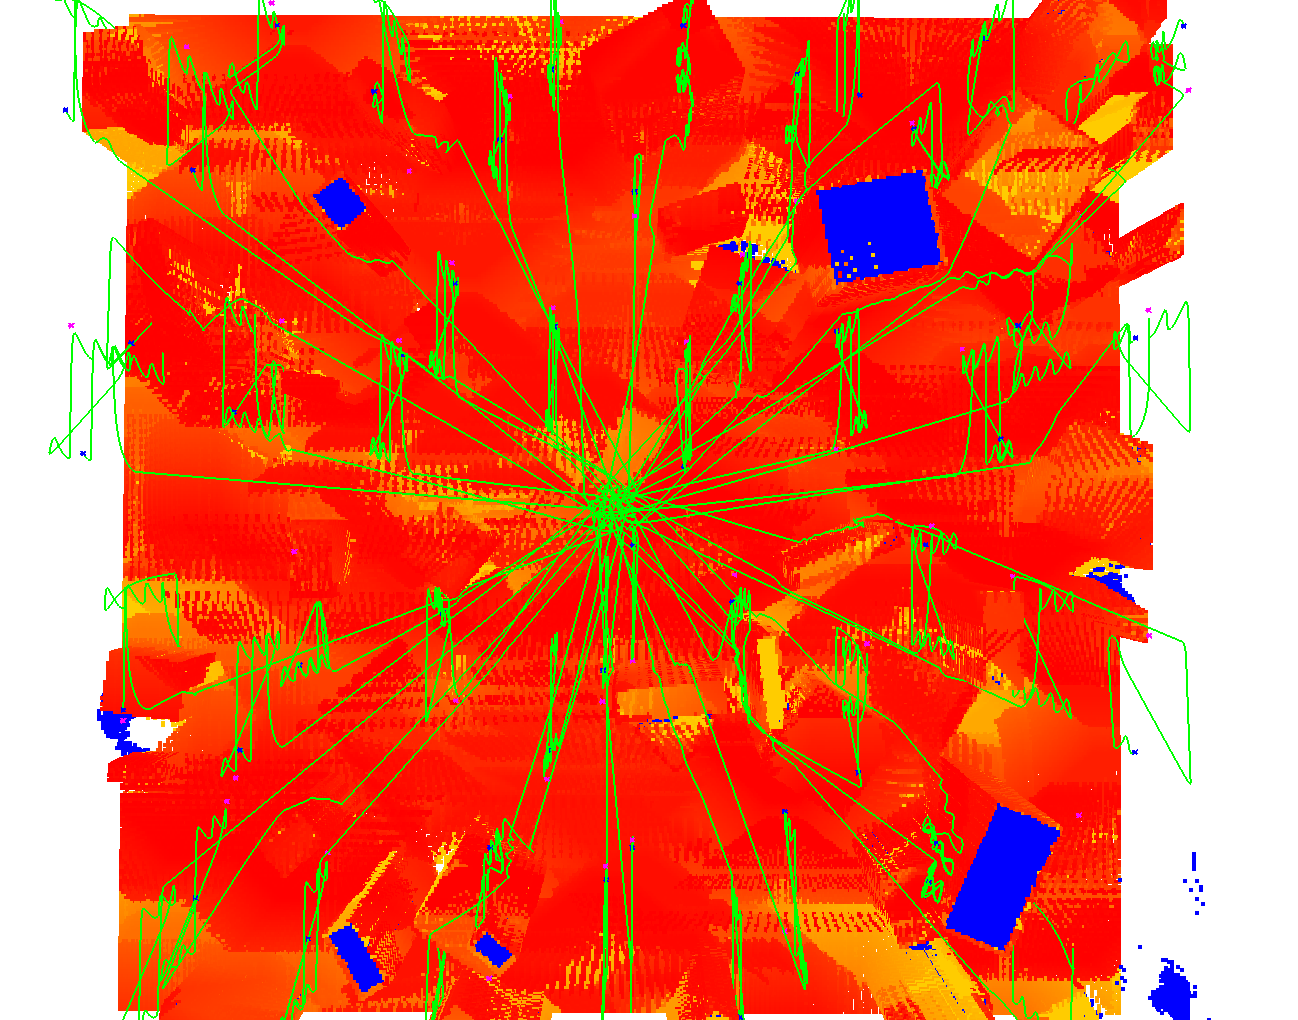
\includegraphics[width=.3\linewidth]{s50s_map1.png}
    \end{center}
    \vfill

    Состояние карты на конечный момент моделирования, вид сверху
    (слева направо: случайный выбор, поиск неизведанного сектора, 
    распределение по сетке)
    \vfill

\end{tslide}

\begin{tslide}{Результаты экспериментов}

    \centering
    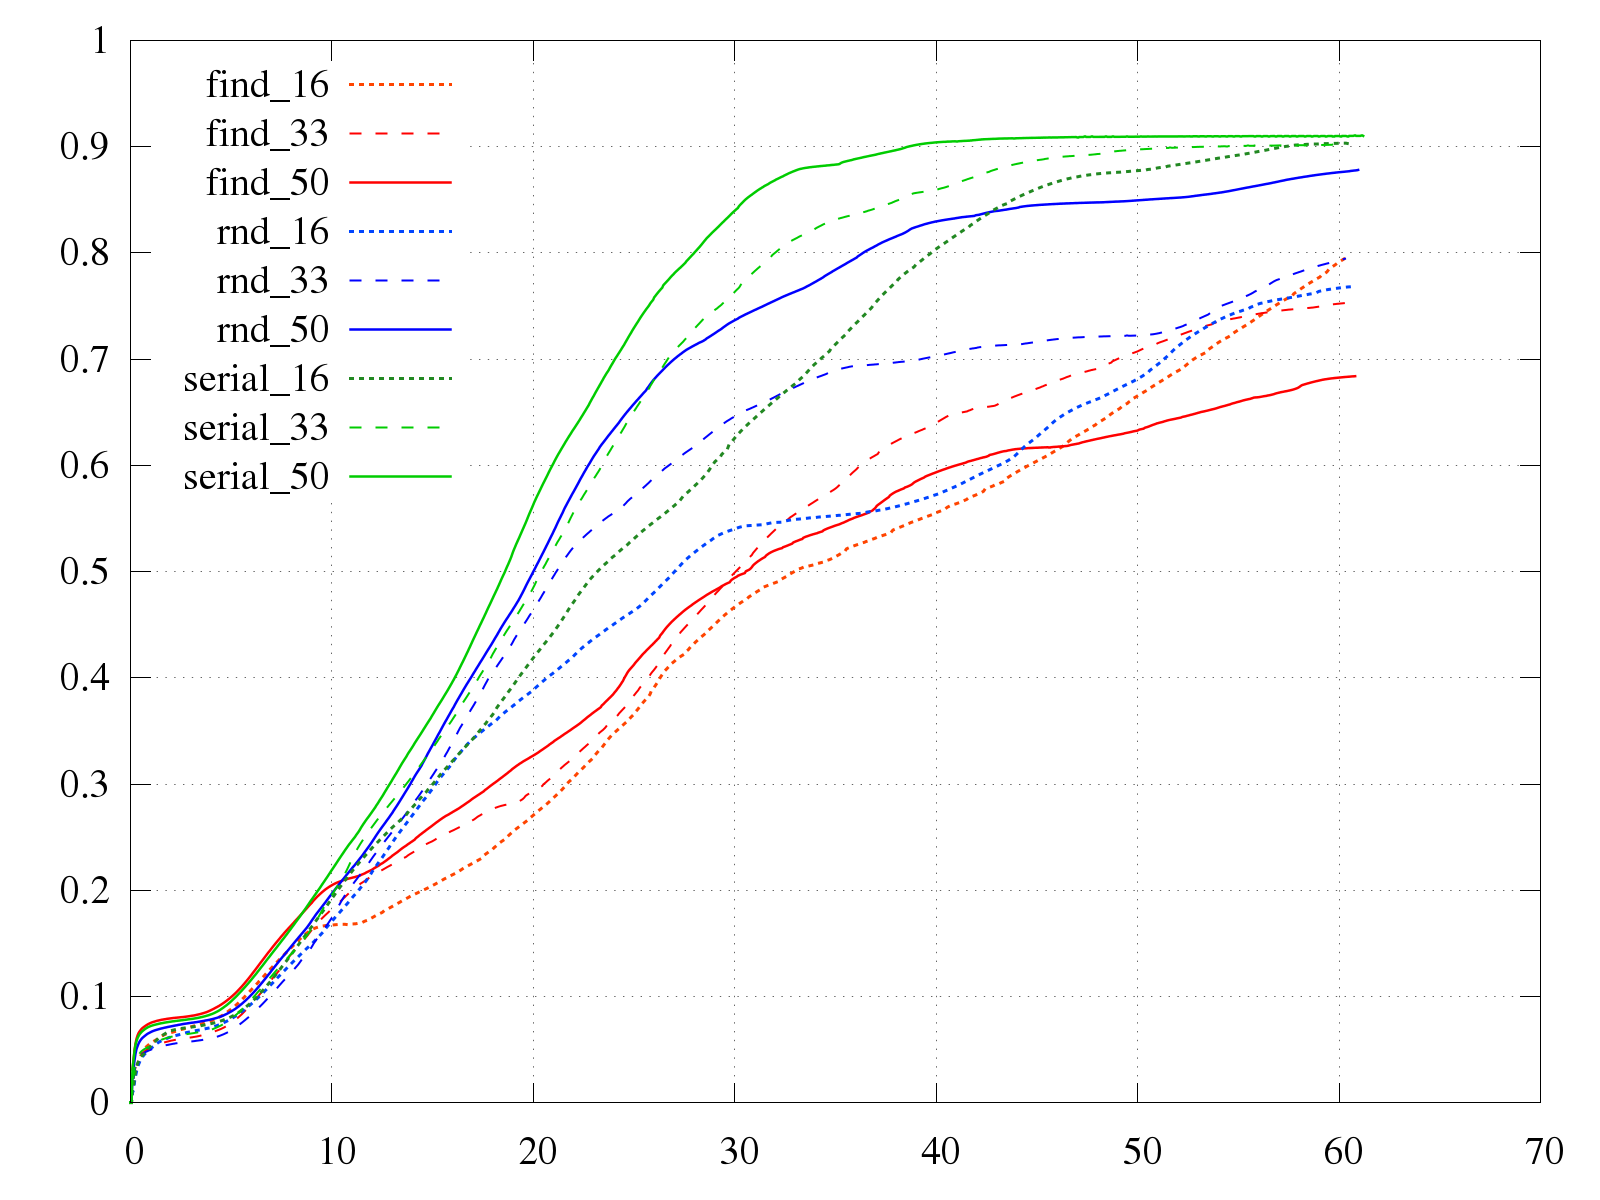
\includegraphics[width=.9\linewidth]{all_pknown.png}
\end{tslide}

\begin{tslide}{Результаты экспериментов}

    \centering
    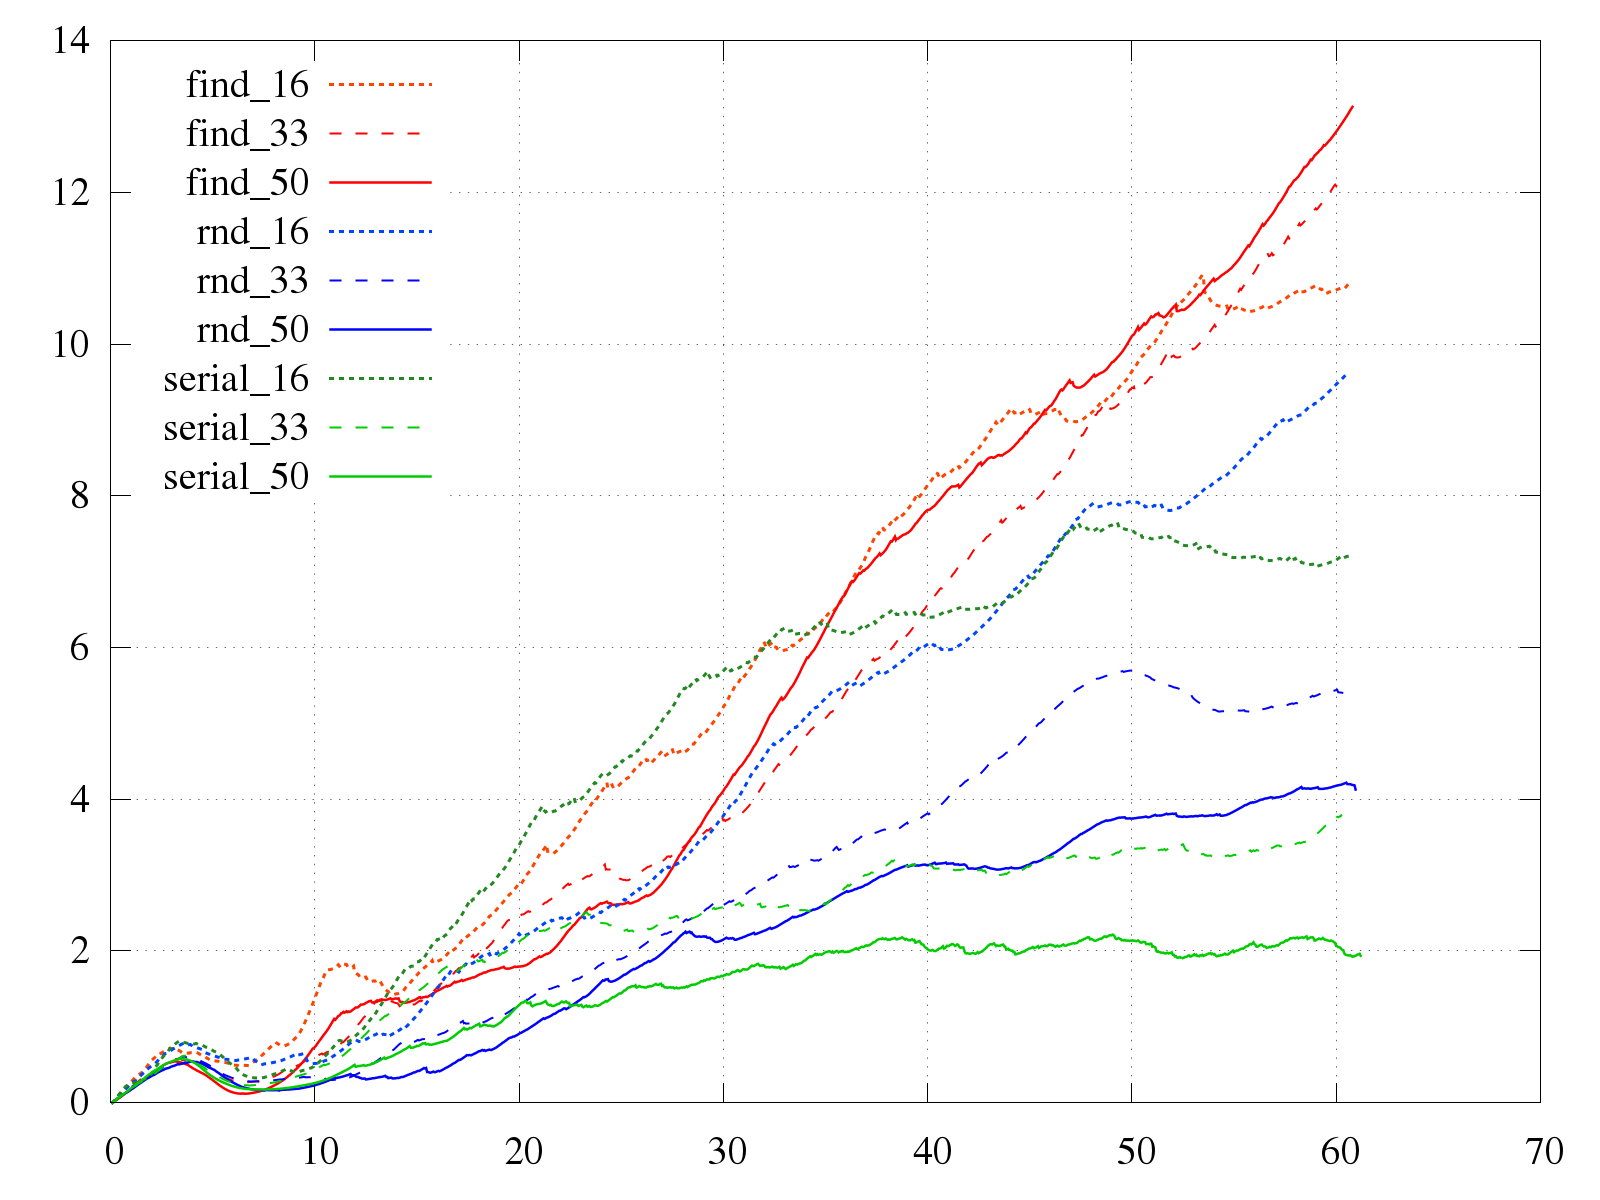
\includegraphics[width=.9\linewidth]{all_ts.png}
\end{tslide}

\begin{tslide}{Выводы}

    В процессе выполнения работы были достигнуты поставленные цели:
    \begin{mintemize}
    \item Разработан алгоритм обследования местности
    \item Написано ПМО
    \item Произведены эксперименты
    \item Проанализированы результаты
    \end{mintemize}

\end{tslide}

\begin{cslide}
    \LARGE Спасибо за внимание.
\end{cslide}

\end{document}
